\section{Herramientas para manipular ficheros DWG.}

Se ha establecido como requisito inicial que el proceso de extracción sea desarrollado con tecnología Java, dado que es una tecnología fiable y muy extendida y compatible con múltiples plataformas hardware / software. 

Con este requisito, se ha realizado una búsqueda de todas las herramientas disponibles en el mercado, libres / propietarias, gratuitas / con licencia, que permiten el manipulado, en modo lectura al menos, de un fichero con formato DWG. En esta búsqueda se han identificado las siguientes alternativas:

\begin{itemize}

\item{RealDWG \cite{RealDWG}: librería licenciada por la propia empresa AutoDesk para desarrollar software que pueda trabajar con ficheros DWG de una forma sencilla y documentada. Tiene un coste de licencia elevado, sobre los 5.000 dolares, y el proyecto en el que vaya a ser utilizada debe ser validado y autorizado por la propia empresa AutoDesk.}

\item{LibDWG \cite{LibDWG}: librería de código abierto desarrollada en lenguaje C que en teoría permite el acceso en modo lectura a un fichero DWG. El desarrollo de la misma se detuvo en Julio del 2009 y no existe una versión estable ni documentación ni ejemplos suficientes para su utilización.}

\item{LibreDWG \cite{LibreDWG}: librería de código abierto desarrollada por la comunidad GNU y basada en los desarrollos anteriores de LibDWG. El desarrollo de la misma esta en una fase alpha, no estable aún, y no existe una API correctamente documentada para trabajar con la misma. También esta desarrollada en lenguaje C.}

\item{DWGDirect \cite{OpenDWG}: librería desarrollada por la <<Open Design Alliance>>. Esta librería solo esta accesible para socios de la organización.}

\end{itemize}

Las conclusiones de la búsqueda no son muy satisfactorias. No parece existir una alternativa real y consolidada más allá de licenciar a la propia compañía AutoDesk el kit de desarrollo RealDWG. Ninguna alternativa de las mencionadas anteriormente contempla Java como tecnología a utilizar.

La <<Open Design Alliance>> no publica su librería para trabajar con ficheros DWG fuera de sus socios y miembros pero sin embargo publica y libera periódicamente una especificación del formato interno del fichero DWG. Esta especificación se obtiene a través de mecanismos de ingeniería inversa. La última especificación disponible aparentemente da soporte a los formatos del fichero DWG desde la versión 13 de AutoCAD hasta las versiones 2010-2012. 

Analizando la situación se opta por desarrollar un interprete nativo en Java, siguiendo las especificaciones publicadas por la <<Open Design Alliance>>. Tras aproximadamente 30 horas de desarrollo, empieza a ser una realidad que esta elección no es la mejor, dado que las especificaciones son complejas, incompletas y va a requerir mucho más tiempo del planificado, desarrollar una librería Java capaz de interpretar mínimamente un fichero con formato DWG. En este punto se esta analizando todavía la cabecera del fichero DWG, tratando de identificar con la ayuda de un editor hexadecimal, los diferentes campos que según la especificación debe contener el fichero. Más alla de estas dificultades, el proyecto a estas alturas acumula un retraso importante respecto a la planificación inicial porque durante los meses de Enero, Marzo y Abril 2012 el proyecto esta detenido por falta de disponibilidad de tiempo del alumno. A continuación se muestra el cronograma final con las diferentes tareas y el tiempo de dedicación a cada una de ellas:

\begin{figure}[H]
\begin{center}
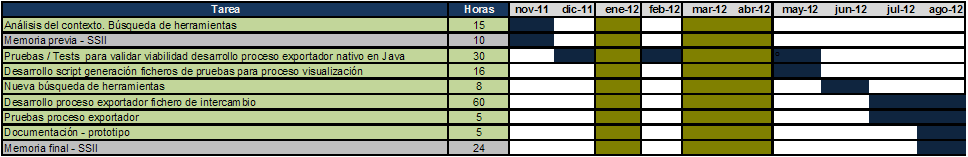
\includegraphics[width=0.95\textwidth]{imgs/schedule}
\caption{Cronograma final del proyecto de SSII.}
\end{center}
\end{figure}

Llegado este punto, se realiza una nueva valoración de las alternativas ya expuestas anteriormente. Se valora la posibilidad de trabajar con la librería LibreDWG, aunque no sea bajo la tecnología Java, dado que lo importante para el proyecto es ser capaces de extraer la información del fichero DWG y ponerla a disposición de otros sistemas informáticos en un formato legible y sencillo de tratar. La tecnología debe ser un medio y no un fin en si mismo. Una vez tomada la decisión de abandonar Java como lenguaje de programación, se realiza una nueva búsqueda y se encuentra una posible alternativa no localizada en la primera selección de herramientas. 

Se localiza la librería ObjectARX \cite{ObjectARX}, librería proporcionada por la propia compañía AutoDesk para el desarrollo de plugins para su colección de herramientas, incluyendo el propio AutoCAD. Esta librería la ofrece Autodesk sin ningún coste de licencia dado que los productos generados con la misma sólo pueden ser utilizados si se dispone de una herramienta original de AutoDesk con la correspondiente licencia. Permite el desarrollo de los plugins en lenguaje C++ y en lenguajes disponibles en la plataforma .NET (C\# y VB .NET). Y lo mas importante, proporciona una API bien documentada y estable para el acceso y manipulado de ficheros DWG.

Dado que el formato DWG y el AutoCAD son un estándar de facto en el sector de las infraestructuras aeronáuticas, se establece como requisito previo que los usuarios finales del proceso extractor dispongan del propio software AutoCAD. Por ello, finalmente, se decide desarrollar el proceso extractor como un plugin que trabajará directamente en la propia herramienta AutoCAD y será desarrollado con tecnología .NET, en concreto C\#. 

Estos nuevos requerimientos difieren técnicamente de los inicialmente propuestos pero dada la escasa viabilidad del planteamiento inicial se ha procedido a buscar una solución que permita obtener resultados completamente funcionales y adaptar los requisitos técnicos a la propuesta más viable.

